\chapter{Business architecture}
\label{sec:business-architecture}
	
	This chapter addresses the business architecture of the initiative to model LAM data. The aim is to describe the internal processes, events and roles answering questions concerning WHO shall do WHAT and WHEN.
	
	This chapter first presents the decontextualised architecture specific to LAM modelling initiative and then proceeds to place the management of the LAM asset in the context of a lifecycle model.
	
	However, the description starts by explaining how a prototypical business architecture is structured and that will serve as a framework to better understand the diagrams in this chapter.
	
	\section{Prototypical business structure}
	
	Following the metaphor of layers presented in the motivation view (see Section \ref{sec:how-to-motivation}), the organisation of business structure is also explained in terms of layers. Figure \ref{fig:business-structure-protopypical} depicts three layers with the most important elements of the business structure. 
	
	\begin{figure}[h]
		\centering
		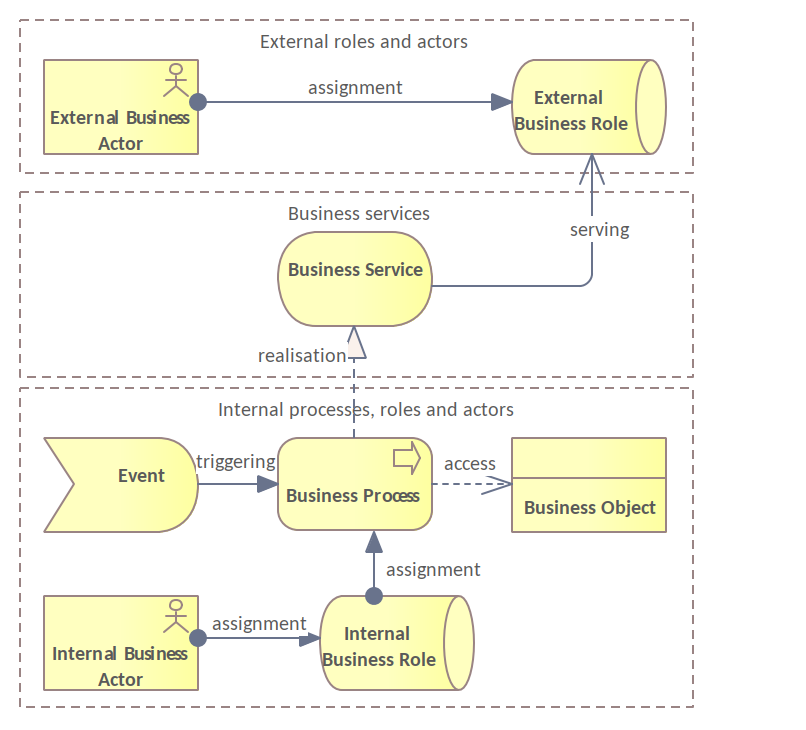
\includegraphics[width=0.78\textwidth]{images/views/Business view.png}
		\caption{The prototypical business structure view}
		\label{fig:business-structure-protopypical}
	\end{figure} 
	
	The topmost layer accounts for the external players or \textit{actors}, which represent a business entity that is capable of performing behaviour and \textit{roles}, which represent skills and responsibilities for performing specific behaviours, and to which an actor can be assigned \citep{archimate3.1}. 
	
	The middle layer represents the \textit{services} that are offered by the organisation to external players. A business service represents explicitly-defined behaviours that a business role, business actor or business collaboration exposes to its environment \citep{archimate3.1}.
	
	The lower layers accounts for the internal organisation in terms of \textit{events}, \textit{roles}, \textit{processes} and \textit{objects}. The business process represents a sequence of business behaviours that achieves a specific result such as a defined set of products or business services. The business event represents an organisational state change; while a business object represents a (passive) concept used within a particular business domain.
	
	\section{Actors and roles}
	\label{sec:actors-roles}
	
	This section describes identified actors and roles relevant to the context of LAM data dissemination. Figure \ref{fig:organisation-structure} depicts their relations.
	
	\begin{figure}[!h]
		\centering
		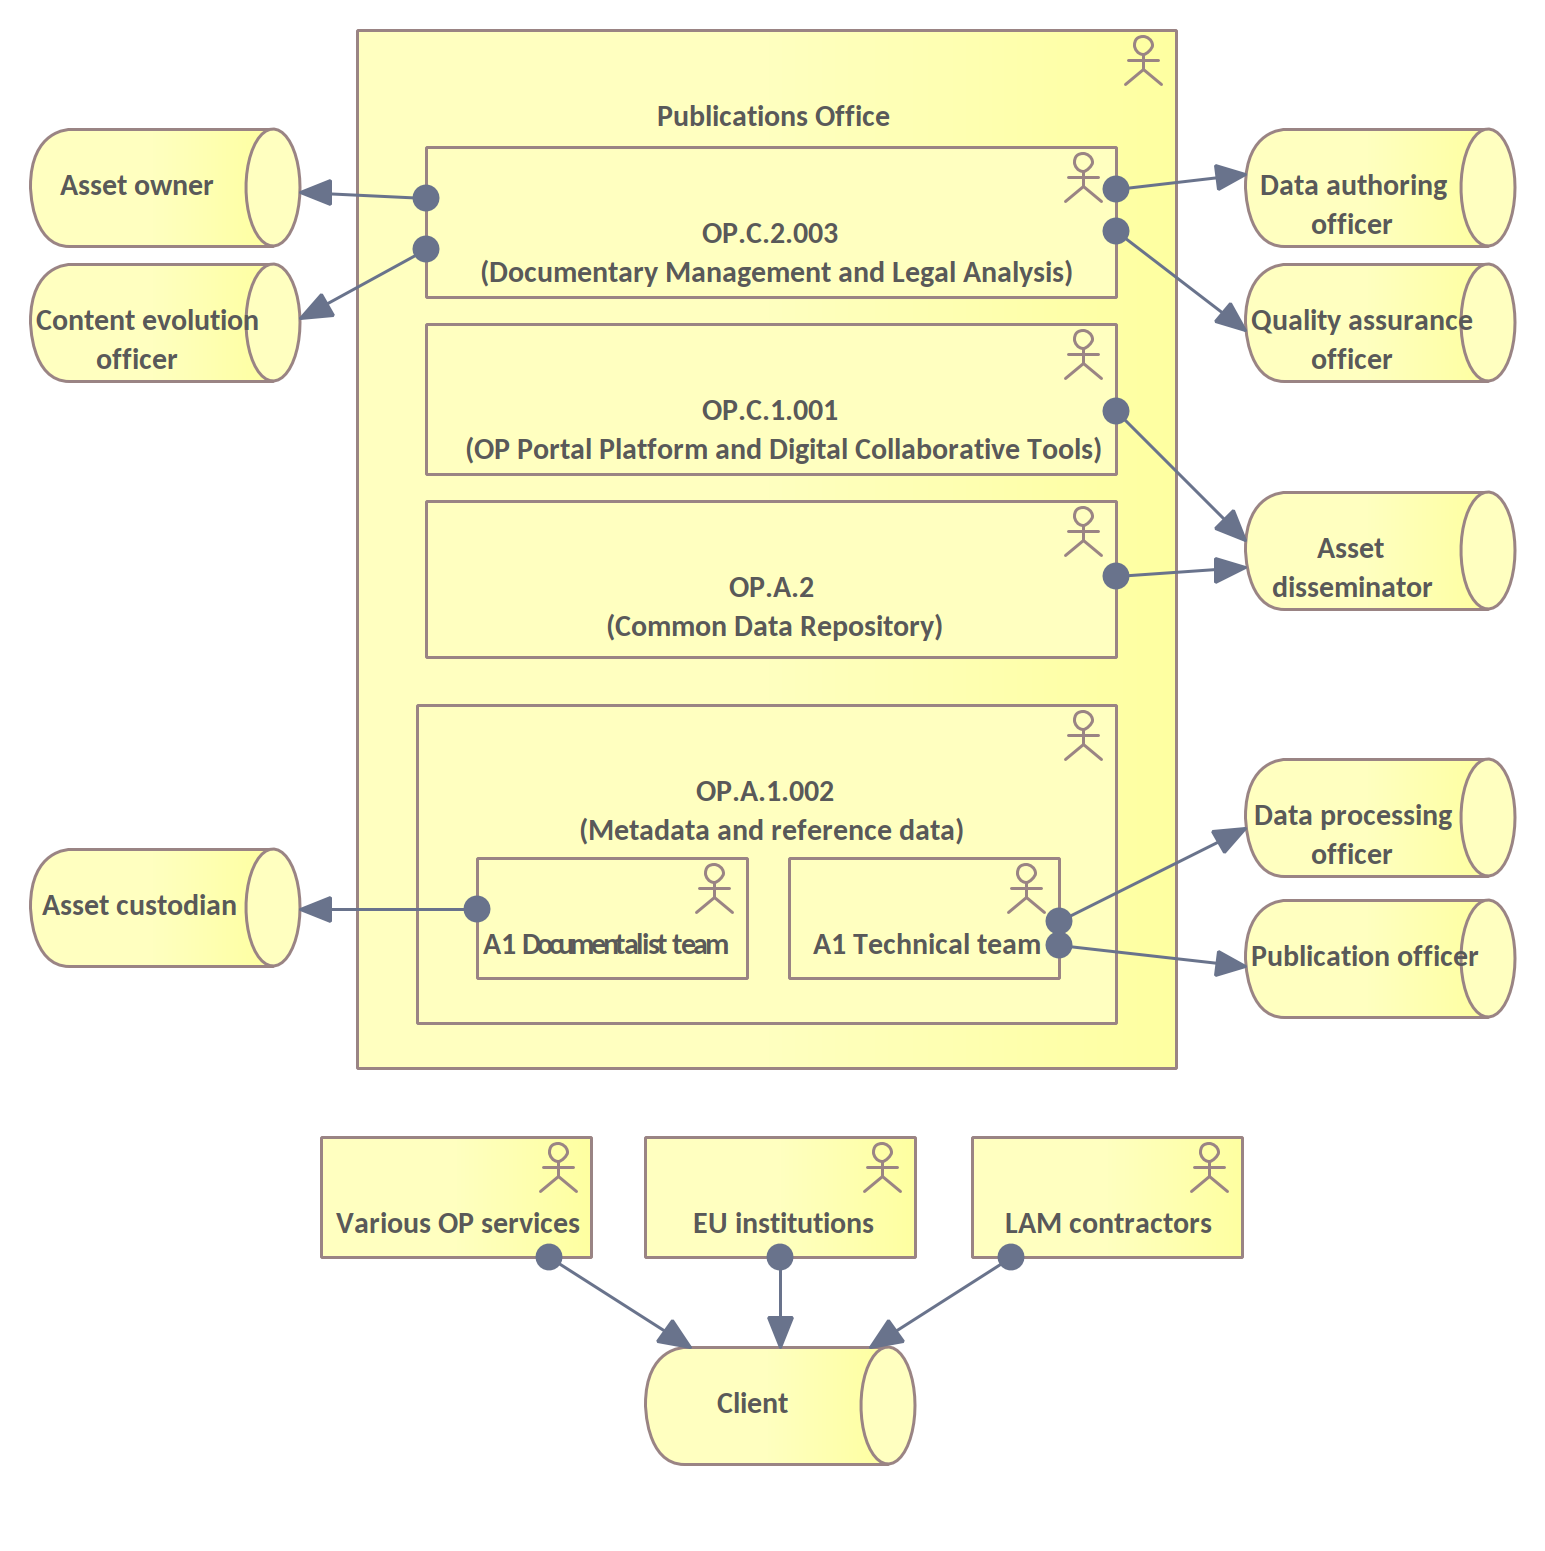
\includegraphics[width=0.995\textwidth]{images/business/Organisation.png}
		\caption{The involved actors and their roles in the LAM data lifecycle}
		\label{fig:organisation-structure}
	\end{figure} 
	
	The OP is a stakeholder in the project but does not have a direct role in the business processes, rather it serves as a frame of reference for the other actors. 
	
	The \textit{Documentary Management and Legal Analysis sector (OP.C.2.003)} at the OP is the project initiator and has a central role to play in the business process. It plays the roles of asset owner, content evolution, data authoring and quality assurance officer. It is not yet decided whether it will play the role of the asset manager or if this role will be transferred to the Metadata and Reference Data sector, who is also the data custodian.
		
	The \textit{asset owner} has accountability for the asset content throughout its life cycle, including decision making authority for creating, classifying, restricting, regulating and administering its use or disclosure. The implementation of these decisions can be delegated.
	
	The \textit{content evolution officer} is the interface with the client collecting change requests, assessing business needs and translating them into data management requirements, all being summarised and documented case-by-case.
	
	The \textit{data authoring officer} (informally referred to as the \textit{editor}) is responsible for editing data in a content management system implementing the cases prepared by the request manager. This is a business role that is responsible for implementing the request case specifications by modifying the data asset accordingly with the provided tools.
	
	The \textit{quality assurance officer} (informally referred to as the \textit{validator}) is a business role that is responsible for ensuring the request case implementation is complete and correct. This role has a special importance and contributes to applying the four eyes principle in the asset lifecycle. Quality assurance officers validate that the content implementation is correct from both technical and business points of view.
	
	The \textit{Metadata and Reference Data sector (OP.A.1.002)} at the OP offers the technical support for LAM data lifecycle management, including editing, validation capabilities, and publication on the dissemination platforms. Because it offers business services and technical services, the actor is split into two sub-components: \textit{the documentalist team} to act as asset custodian and correspondingly \textit{the technical team} taking the role of data processing and publication officer.
	
	The \textit{asset custodian} (informally referred to as the \textit{asset manager}) operates as a trustee on behalf of the asset owner and is responsible for data content, context, and associated business rules. This role ensures the development and enforcement of standards for data within their care.
	
	The \textit{data processing officer} is a technical role that is responsible for preparing the assets for publication and distribution on various channels. The responsibilities include, but are not limited to, data storage, manipulation, automatic transformation and generation of validation and assessment reports.
	
	The \textit{publication officer} is a technical role responsible for packaging and disseminating assets to specialised platforms. This role may also include preparation of release notes and impact assessment preparation. 
	
	The OP Portal website is the main dissemination channel for the human readable representation of LAM data. The sector in charge of \textit{OP Portal Platform and Digital Collaborative Tools (OP.C.1.001)} play the role of the main asset disseminator. 
		
	The \textit{Common Data Repository unit (OP.A.2)}, in charge of Cellar system \citep{cdm-francesconi2015ontology} also plays the role of asset disseminator because the machine readable representation of the LAM data is published in the Cellar system.
	
	The \textit{asset disseminator} role provides with reliable data the dissemination capabilities which are meant to make assets available for the clients. The dissemination of assets is done either in human readable or in machine readable representations.
	
	The LAM contractors, various EU institutions and OP services have been identified already in the motivation structure section (see Section \ref{sec:motivation-architecture}) as stakeholders. From the business point of view these stakeholders are agents playing the role of a client.
	
	The \textit{client} (either the change requester and or the data user) is a generic external role who, on the one hand, consumes data and services provided by the asset owner and, on the other hand, suggests creation and publication of new assets or modification of existing ones.
	
	\section{Maintenance of semi-structured LAM data}
	\label{sec:maintenance-of-excel}
	In a previous project dealing with creating a model for the LAM data (internally referred to as LAM\#1 \citep{lam-preliminary-requirements-2019}) a set of artefacts and a data management methodology was created in order to aid the LAM management team to organise and edit the data. 
	
	\begin{figure}[h]
		\centering
		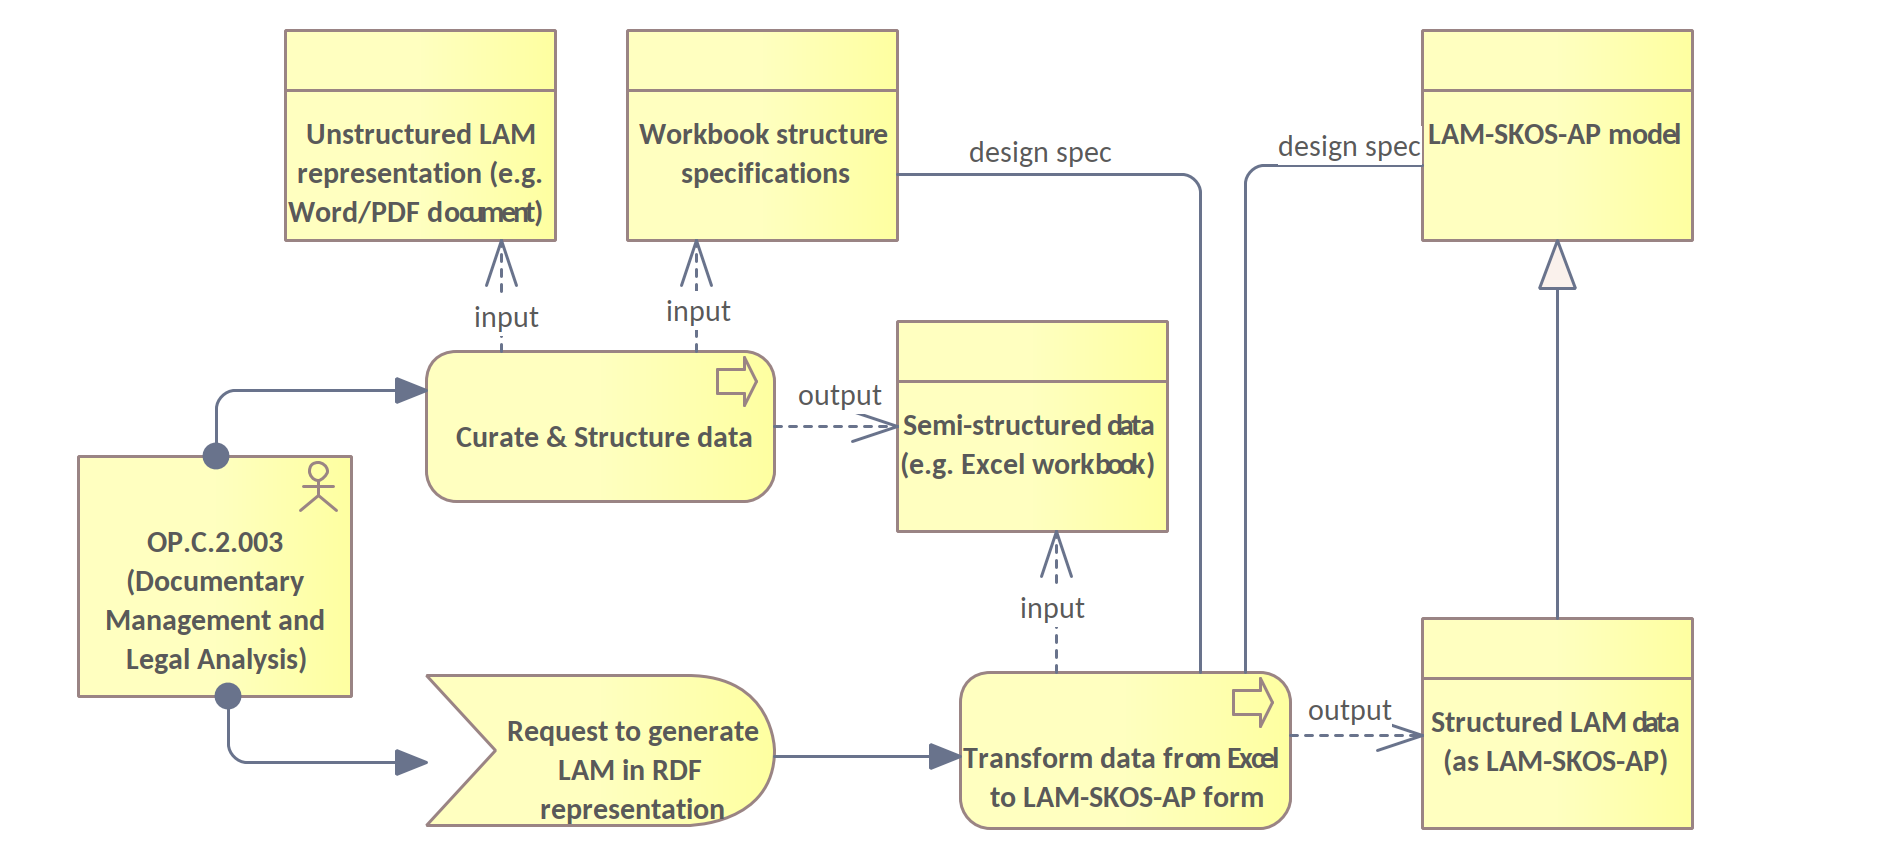
\includegraphics[width=0.995\textwidth]{images/business/context/post LAM1 context.png}
		\caption{The maintenance of LAM data in the semi-structured form}
		\label{fig:post-lam1-context}
	\end{figure} 
	
	After the LAM\#1 project \citep{lam-preliminary-requirements-2019} was completed three new capabilities were added to the LAM team: (a) management of LAM data in a semi-structured representation (in an Excel workbook \cite{excel}) thanks to a specification on how to structure the workbook \citep{lam-excel-structure-2019}, (b) the possibility to transform the LAM data into RDF representation following the LAM-SKOS-AP \citep{lam-skos-ap-2019} model specifications  and (c) uploading and editing the LAM data in the VocBench3 system \citep{stellato2017towards,stellatovocbench}. Figure \ref{fig:post-lam1-context} depicts this situation. 
	
	Over time, the LAM team (the actor on the left side of the diagram) performs the curation and structuring of the LAM data producing the Excel workbook (semi-structured representation). As the first input to this process, the team relies on the existent Word documents describing Eur-Lex LAM structure in human readable form \cite{lam-eurlex-spec-2017} and the second input is the specifications for structuring the Excel \mbox{workbook \citep{lam-excel-structure-2019}}. 
	
	When a satisfiable version of the semi-structured data is available, the LAM team requests generation of the RDF representation for it. The reason behind this is to ultimately migrate toward editing LAM data in VocBench3 \citep{stellato2017towards} and away from Excel \cite{excel}. 
	
	In the past, this transformation was performed by the contractor. Now this may be transferred to the Metadata and Standardisation Unit or continue using the contractor for technical support. This is necessary because the transformation is not a one time operation but continues over a period of time as both the data and the generation script need to pass through a series of evolutions before arriving at a stable RDF representation. 
	
	The transformation output is the LAM data instantiating LAM-SKOS-AP \mbox{model \citep{lam-skos-ap-2019}}. The instantiation relationship is depicted in Figure \ref{fig:post-lam1-context} through a realisation connector from Structured LAM data business object to the LAM-SKOS-AP model business object. 
	Next section explains how the LAM data is maintained and published in RDF representation. 
	
	\section{Maintenance and publication of structured LAM data}
	\label{sec:lam-maintenance-publication}
	
	Ultimately, the LAM data shall be maintained in LAM-SKOS-AP representation using VocBench3 system. This is depicted in upper part of Figure \ref{fig:lam2-context}.
		
	\begin{figure}[!h]
		\centering
		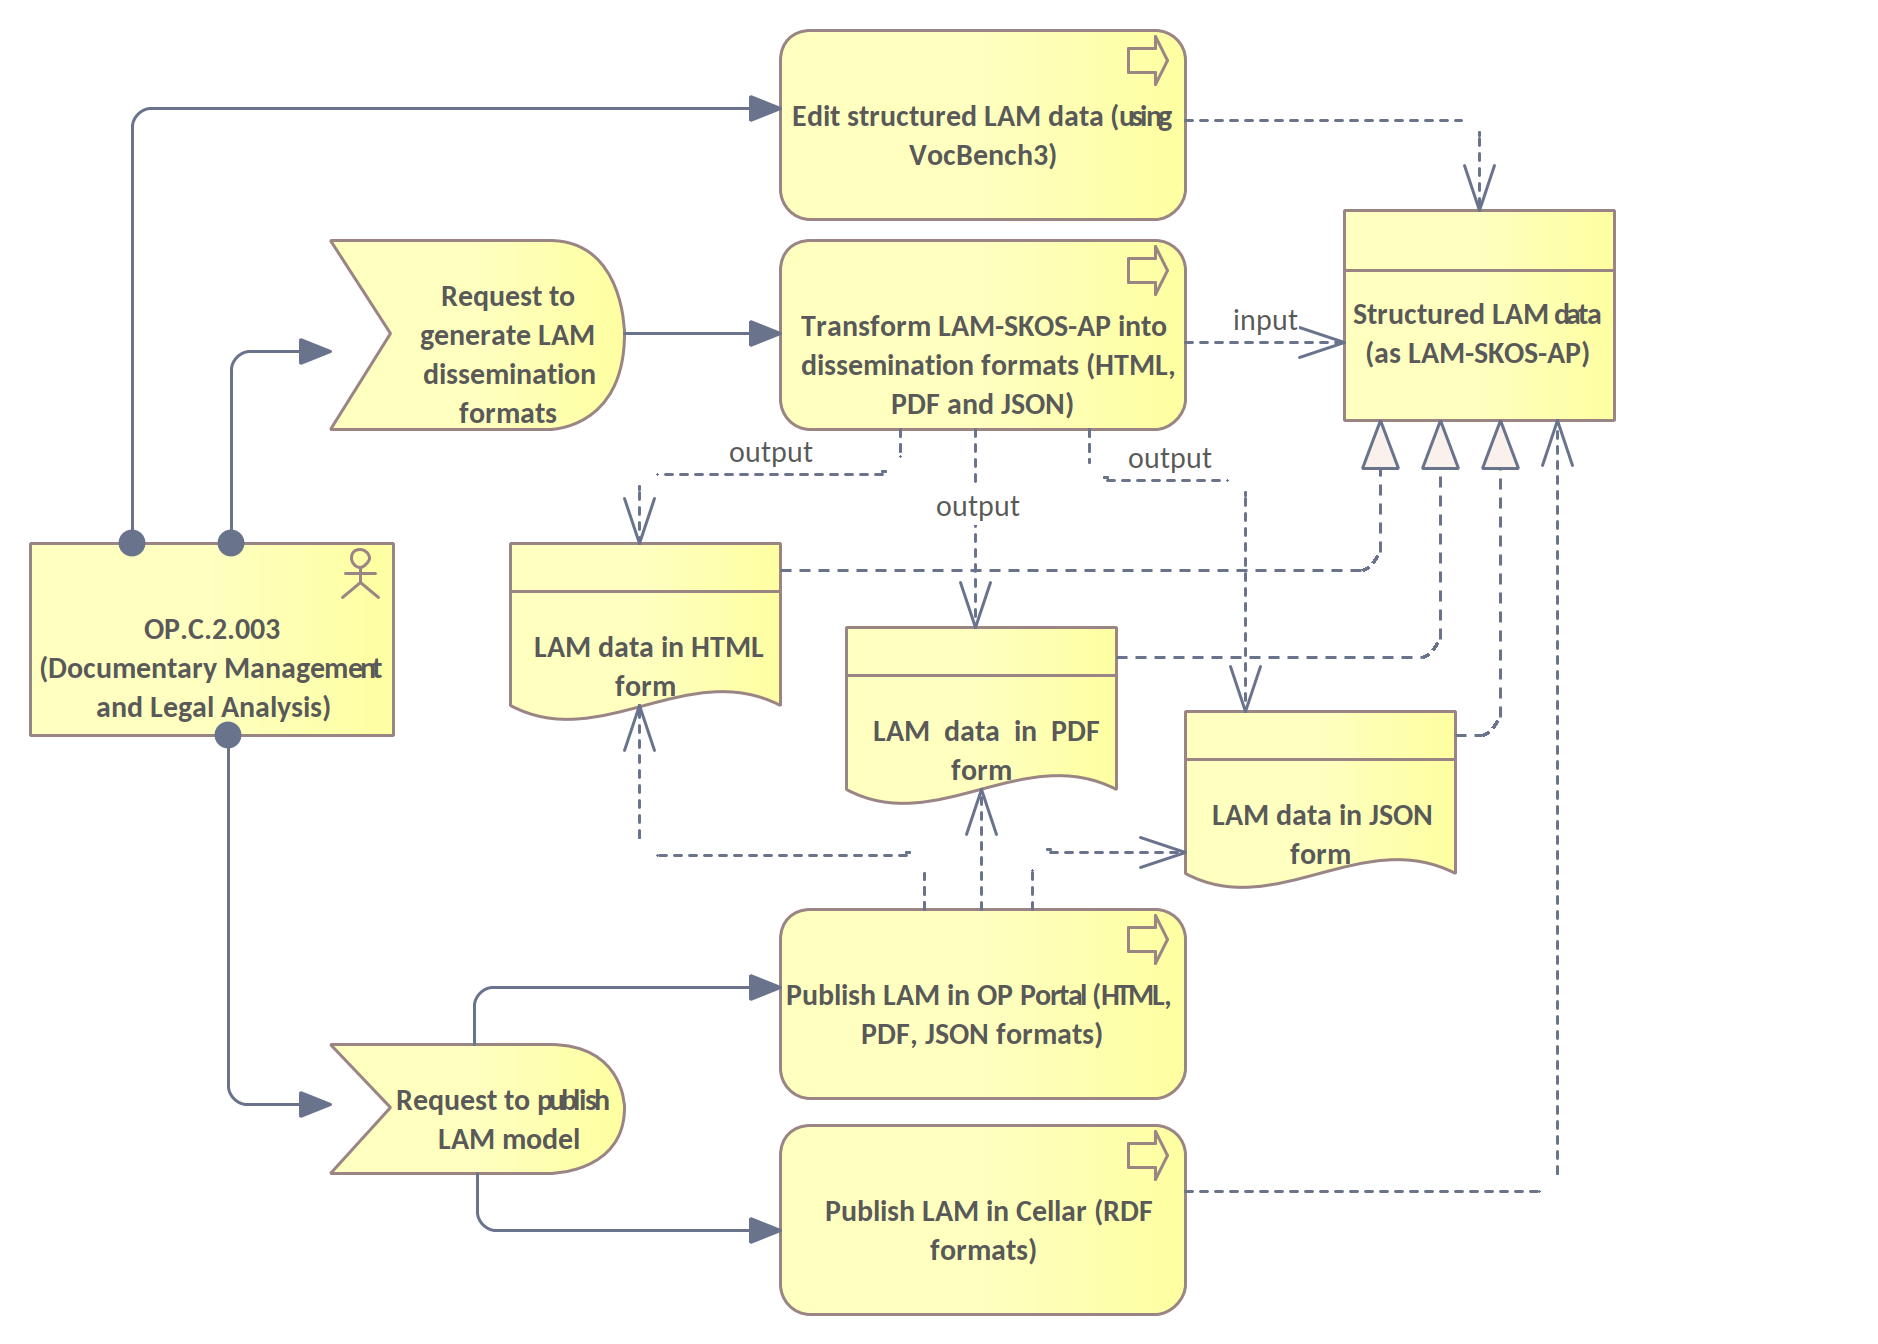
\includegraphics[width=0.95\textwidth]{images/business/context/LAM2 context.png}
		\caption{The publication architecture for LAM data}
		\label{fig:lam2-context}
	\end{figure} 
	
	When a stable version of the data is achieved, it can be published for dissemination to the clients. To do so, a request to generate dissemination formats is issued by the LAM team, which will trigger the transformation process from LAM-SKOS-AP into HTML, PDF and JSON representation forms, which are human readable. This is depicted in the central part of Figure \ref{fig:lam2-context}. 
	
	The human readable dissemination forms need to be validated and assessed for publication. After which the LAM team issues a new request to publish the data on the dissemination platforms. This triggers two processed: the first one is to publish the human readable representations into OP Portal and the other to publish the LAM data in LAM-SKOS-AP, the machine readable representation in Cellar. 
	
	The responsible agent for running these processes is the OP Metadata and reference data sector (OP.A.1.002). This shall be organised in an internal agreement at the OP. Moreover, the management of LAM data should be aligned with the practices and methods implemented by OP.A.1.002. These practices are internally known as asset lifecycle process and are briefly presented in the next section. 
	
	\section{Asset lifecycle process}
	\label{sec:asset-lifecycle}
	
	The previous sections presented the processes and business object specific to the context of LAM\#2 project. These processes, however, need to be viewed from a data management perspective. This leads to the need to adopt a data management methodology. 
	
	This section presents the overview of the asset lifecycle process applicable to LAM data. This lifecycle process is adopted from the A1 unit, which is in the business of semantic asset management and publication. The diagram summarising the lifecycle process is provided in Figure \ref{fig:lifecycle-overview}. 
	
	\begin{figure}[!h]
		\centering
		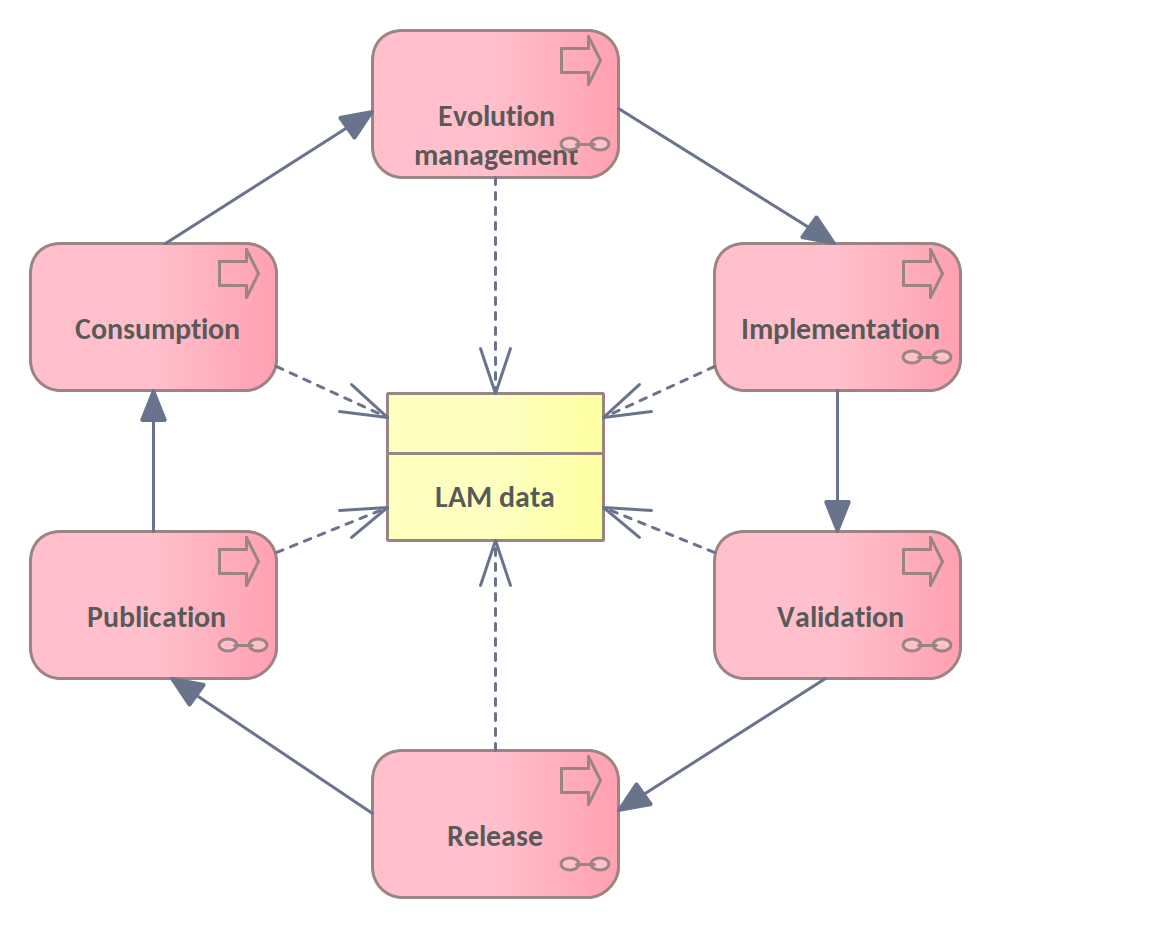
\includegraphics[width=0.73\textwidth]{images/business/lifecycle/Lyfecycle overview.png}
		\caption{The baseline business architecture of LAM data}
		\label{fig:lifecycle-overview}
	\end{figure} 

	The asset lifecycle process is organised in six stages: \textit{evolution management}, \textit{implementation}, \textit{validation}, \textit{release}, \textit{publication} and \textit{consumption}. Each of the stages represents a business sub-process accessing the LAM data object positioned centrally in Figure \ref{fig:lifecycle-overview}.
	
	The \textit{evolution management} stage deals with management change request cases. This stage also includes recording, analysis, negotiating back with the client and then finally deciding and planning the implementation of change request cases.
	
	The \textit{implementation} stage deals with performing the actual changes in the LAM data implementing one case at a time and verifying that the modifications reflect the original client request.
	
	The \textit{validation} stage follows the implementation and is performed by a different actor than the one performing the implementation process. Having the validation done by a second pair of eyes enforces the ``four eyes principle'' adopted by the OP in the proofreading and other authoring tasks. 
	
	The \textit{release} stage deals with all data transformations and preparation of artefacts to be disseminated and consumed by the final clients. 
		
	The \textit{publication} stage deals with packaging the content and disseminating it to the selected data disseminators, OP Portal and Cellar being the main ones. During this stage a set of announcements and communications ensure that the main stakeholders and the broad public are aware of the published new version of the asset.
	
	In the \textit{consumption} stage only external actors are involved acting as clients. During this phase the data is accessed and used as necessary by each of the clients. While using the data assets, clients come up with additional requests for either changing content of the existent assets or adding and publishing new ones.
	
	A more detailed description of the stages in the lifecycle process is provided in the document describing the asset publication workflow architecture \citep{costetchi2020d} owned by A1. This architecture document was not yet released to the public so the A1 team shall be contacted for consultation.
	
	\section{Role allocation in the lifecycle process}
	
	This section brings together the actors and roles presented in Section \ref{sec:actors-roles} and the lifecycle process. In Figure \ref{fig:lifecycle-roles} the actors (C2, A1, C1, A2 and others) are represented as swim-lines (see Figure \ref{fig:organisation-structure} for details). 
	
	\begin{figure}[!h]
	\centering
	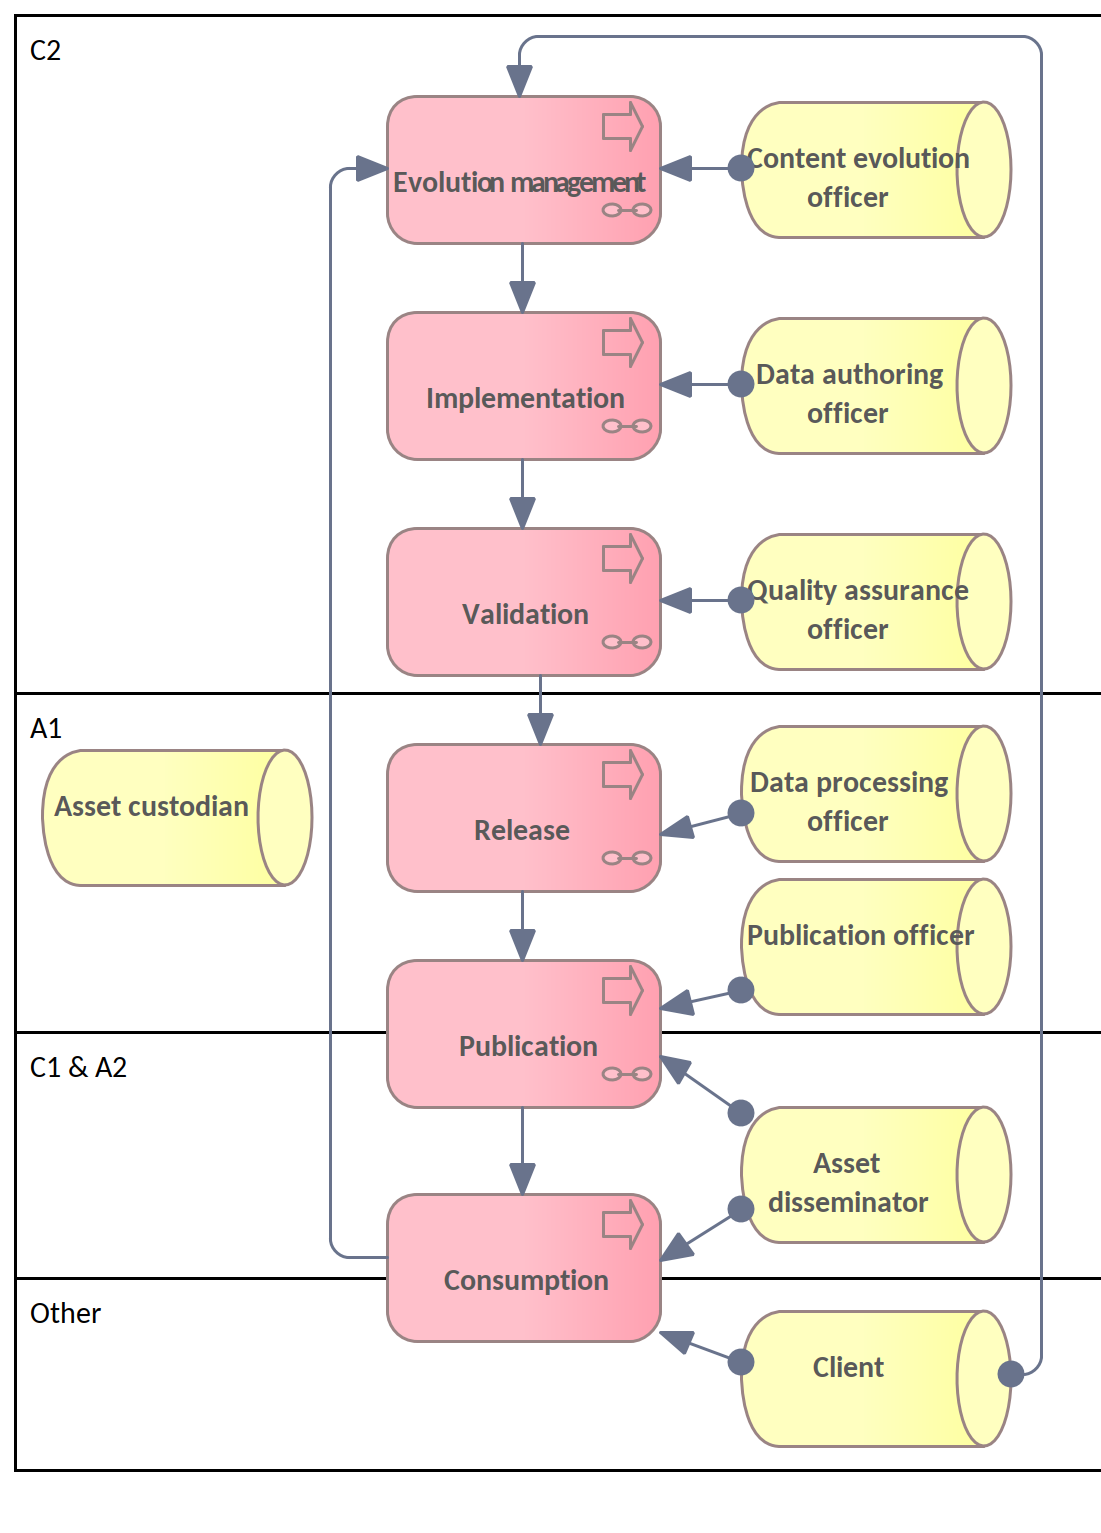
\includegraphics[width=0.69\textwidth]{images/business/lifecycle/Lifecycle roles.png}
	\caption{The lifecycle actors and roles}
	\label{fig:lifecycle-roles}
	\end{figure}

	The process steps are organised top-down, and the roles are associated to each process step. The first three steps: evolution management, implementation and validation are executed by the LAM team in C2 taking consecutively the role of the content evaluation officer, data authoring officer and the quality assurance officer. 
	
	After validation, the release and publication steps are taken on by the A1 technical team who deals with technicalities of data transformation, packaging and transmission to the dissemination platforms. The A1 team takes the roles of data processing officer and that of data publication officer. 
	
	The A1 team also plays the role of asset custodian and is responsible for data content, context, and associated business rules, acting as a trustee on behalf of the asset owner (the C2 unit). This role is involved in overseeing the whole lifecycle process and ensuring its proper execution. The reason why this role is taken by A1 is because this unit provides the technical infrastructure and capabilities for editing, validating, transforming and publishing semantic assets. 
	
	The C1 and A2 units, where the OP Portal team and Cellar teams are situated, play their part partially in the publication and partially in the consumption stages of the lifecycle. They represent the dissemination platforms and, therefore, participate in the asset upload on the one hand and asset access by the clients on the other hand. 
	
	The last swim-line, at the bottom of the diagram, titled ``Other'', includes all the stakeholders (see details in Section \ref{sec:actors-roles}) that play the role of the client and participate in the consumption phase (and, of course, in the evolution management phase, if they send new requests for evolution). 
